%!TEX ROOT = thesis.tex
\chapter{Introduction}
\section{First Test and I need a really long title, please do oblige me won't you? Just a few more words and yes we're there}
\lipsum[1-4]

\begin{figure}[hbt!]\centering
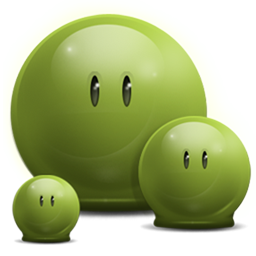
\includegraphics[width=.3\textwidth]{green}
\caption{First figure. OK?}
\end{figure}

\subsection{Second Test}
There are studies on factors blah blah \cite{audibert:2004} and\endnote{This is a footnote, or rather an endnote. Note that footnotes/endnotes are not encouraged in scientific and engineering disciplines.} they are really amazing\endnote{don't you agree?}\cite{budanitsky:hirst:2006}.

\begin{figure}[hbt!]\centering
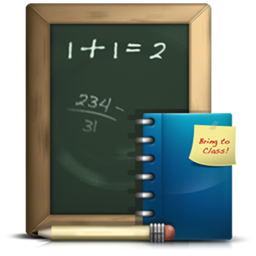
\includegraphics[width=.3\textwidth]{school}
\caption{Second figure. Now I need a long caption to test out how things look in the List of Figures. Is this long enough yet? Is it? Is it?}
\end{figure}

\section{Yeah}
\lipsum[5-6]

\begin{table}[hbt!]
\caption{This is a table}
\centering
\begin{tabular}{ l c r }
\hline
Hey & How's it & Going?\\ \hline
Fine! & Just great. & See ya!\\
Fine! & Just great. & See ya!\\
\hline
\end{tabular}
\end{table}